\section{O Que São Aquisições Sísmicas e Como Modelá-las}

	No ramo da mineração, não se pode tentar a esmo a descoberta de recursos
	minerais no subterrâneo de um local em que se já se suspeita sua existência.
	Do contrário, tal processo imprudente levaria a um alto custo monetário.
	É necessário que, de alguma forma, se obtenha a forma dessa estrutura oculta
	para se saber os pontos onde se encontram as jazidas/poços desse recurso.
	A obtenção dos dados de como é essa estrutura se chama \textbf{aquisição
	sísmica}.

	A forma de se realizar essa aquisição pode variar com o ambiente e os
	métodos adotados para coleta de dados e processamento dos mesmos. Os
	recursos minerais desejados podem se encontrar tanto em meios terrestres
	e/ou subaquáticos. Contudo, o meio em que a aquisição será realizada pouco
	importa nesse trabalho.

	Para a coleta dos dados a serem processados podemos citar dois exemplos
	de aquisição
	\begin{enumerate}
		\item \textbf{marítima}: um navio equipado com um canhão
		sonoro emite ondas sonoras cujas reflexões e refrações nas camadas
		terrestres submarinas são captadas por filas de hidrofones puxadas pelo
		mesmo navio.
		\item \textbf{terrestre}: um explosivo é (preferencialmente) enterrado
		em um terreno. Sua explosão gera uma onda sonora cujas
		reflexões são captadas por geofones distribuídos relativamente próximos,
		na superfície.
	\end{enumerate}
	
	Costuma-se alterar a posição da fonte sonora na realização da aquisição para 
	se obter mais dados de como aquele ambiente se 
	comporta com o transporte de ondas e, baseando-se nisso, modelar sua estrutura 
	em si.

	Esse recolhimento dos dados consistirá em \textbf{traços}, como se pode ver na Figura 
	\ref{fig:seismic-traces}. Esses consistem em gráficos das amplitudes das ondas sonoras, obtidas através dos hidrofones/geofones, ao longo do tempo. 
	A partir desses traços, detecta-se, por análise técnica, onde se 
	encontram as interfaces entre as camadas do domínio analisado e do que elas são feitas. Nisso consiste o processamento dos dados colhidos.

    \begin{figure}[H]
        \centering
        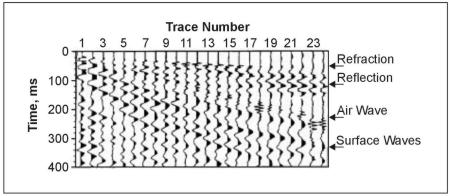
\includegraphics[scale=3.]{chapters/chp2/images/seismic-traces.jpg}
        \caption{Exemplo de traços sísmicos}
        \label{fig:seismic-traces}
    \end{figure}

	Contudo, quanto aos métodos de processamento utilizados, nesse 
	trabalho simularemos um problema
	direto, ou seja, estipulando o meio (nesse caso, não-homogêneo) da aquisição,
	veremos como as ondas se propagam nele. Para tal, usaremos um método
	matemático específico. Nesse trabalho, como já foi dito no Capítulo
	\ref{chp1}, é o de Método de Diferenças Finitas.